% ============================================================
% Section 6: Unified benchmark
% All numbers come from benchmark/results/raw.csv (10 seeds per point),
% d2d_prediction.csv, mismatch_v5.mat and rwp_warmup_v5.mat
% (MATLAB code in benchmark/).
% ============================================================

\section{A Unified Benchmark of Mobility Models}
\label{sec:benchmark}

To separate the factors identified in Section~\ref{sec:effect}, we built one benchmark in which the network, content, requests and caching policies are fixed and only the mobility model changes. Beyond comparing models, we ask which measured property of the mobility determines the gain, so that a result obtained under one model can be carried over to another. The MATLAB code runs unchanged in GNU Octave and is released with the paper.

\subsection{Setup}
\label{subsec:setup}

Table~\ref{tab:params} lists the parameters. Two hundred users move in a 1~km $\times$ 1~km area served by a $5\times5$ grid of small base stations (SBSs), each covering a 200~m $\times$ 200~m cell; a user is associated with the SBS of the cell it is in. Each user sends requests as a Poisson process with rate $1/120$ per second, for files drawn from the Zipf law~\eqref{eq:zipf} with $N=1000$ and $\gamma=0.8$. Each SBS stores $C=50$ files. Each user stores $c=10$ distinct files, drawn with probability proportional to popularity, and can serve peers within 50~m.

A request must be delivered within $T_d=60$~s. Following~\eqref{eq:effhit}, delivery from an SBS needs $D_s=10$~s of uninterrupted association with an SBS that holds the file, and delivery over D2D needs $D_d$ seconds of uninterrupted contact with a peer that holds it, with $D_d$ between 2 and 30~s. A request for a file in the user's own cache counts as offloaded.

\begin{table*}[t]
\centering
\caption{Benchmark parameters}
\label{tab:params}
\footnotesize
\renewcommand{\arraystretch}{1.1}
\begin{tabular}{ll@{\hspace{0.6cm}}ll}
\hline
Parameter & Value & Model & Setting \\
\hline
Area, users & 1~km $\times$ 1~km, $U=200$ & Random walk & New direction every 30~s; reflection at the walls \\
SBSs & $5\times5$ grid, 200~m cells & RWP & Speed $\sim U[0.5v,1.5v]$, pause $\sim U[0,60]$~s \\
Library, popularity & $N=1000$, Zipf $\gamma=0.8$ & Gauss-Markov & $\alpha=0.85$, $\sigma_v=0.3v$, $\sigma_\theta=\pi/4$; steering and reflection at the walls \\
SBS cache, user cache & $C=50$, $c=10$ files & Markov cell & Stay w.p.\ 0.3, else a random neighbor; random point in cell \\
Request rate & $1/120$ per user per second & Manhattan & 100~m blocks; straight 0.5, left 0.25, right 0.25 \\
Deadline $T_d$ & 60~s & L\'evy walk & Tails $\alpha=\beta=1.5$; flights 10--1000~m, pauses 10--1800~s \\
SBS delivery time $D_s$ & 10~s & & \\
D2D range, transfer time $D_d$ & 50~m; 2, 5, 10, 20, 30~s & & \\
Travel speed $v$ & 0.5, 1, 2, 5, 10, 20~m/s & & \\
Measured period, warm-up & 3600~s, 2000~s discarded & & \\
Seeds & 10 per configuration & & \\
\hline
\end{tabular}
\end{table*}

\emph{Mobility models.} We implement seven models from the synthetic and structured families of Section~\ref{sec:models}: static users, random walk, RWP, Gauss-Markov, a Markov chain over cells, a Manhattan grid and a truncated L\'evy walk. The parameter $v$ is the speed while moving. Users that reach a wall are reflected, and movement is interpolated at 1~s resolution so that a reflected path does not cut corners. The L\'evy parameters are illustrative and are not fitted to the traces of~\cite{rhee2011levy}. Trace-driven runs are not included; the code accepts a trace in place of a generator.

\emph{Caching policies.} Three SBS policies are compared.
\begin{itemize}
\item \emph{Most popular (MPC)}: every SBS stores the $C$ most popular files. It ignores mobility.
\item \emph{Mobility-aware (MA)}: a greedy placement that uses the \emph{reach matrix} $\mathbf{W}$, where $W_{bb'}$ is the probability that a user at SBS $b$ at a request instant stays with SBS $b'$ for $D_s$ seconds before the deadline. With $\pi_b$ the share of time spent at $b$ and $x_{b'f}\in\{0,1\}$ the placement, the greedy step maximizes
\begin{equation}
\sum_{b}\pi_b\sum_{f}p_f\Big[1-\prod_{b'}\big(1-x_{b'f}W_{bb'}\big)\Big],
\label{eq:maobj}
\end{equation}
treating visits as independent, until every cache is full. $\mathbf{W}$ and $\pi$ are estimated from an independent run of the same model, as an operator would learn them from history. The scheme is an uncoded relative of the helper placement in~\cite{poularakis2013exploiting}.
\item \emph{LRU}: each SBS runs least-recently-used replacement on the requests it receives and serves only users currently associated with it.
\end{itemize}
D2D caches keep the fixed popularity-proportional placement, so that changes in D2D offloading come from mobility alone. We report the snapshot and effective hit ratios of Section~\ref{subsec:metrics} and the D2D offloading ratio.

\emph{Statistics.} Each configuration runs for one measured hour with 10 independent seeds. Figures show the mean with 95\% confidence intervals; the half-width is at most 0.006 for every hit and offloading ratio. Every run discards a 2000~s warm-up. The warm-up matters for RWP: started with speeds in $(0,2v]$ and uniform positions~\cite{yoon2003rwp}, our RWP at $v=5$~m/s slowed from 2.4~m/s in its first 20 minutes to 1.3~m/s in its fourth hour, and its D2D offloading ratio drifted from 0.29 to 0.25 for $D_d=2$~s and from 0.13 to 0.15 for $D_d=30$~s (three seeds). The benchmark RWP uses a positive minimum speed and the warm-up, and stays at 3.6~m/s.

\subsection{Measured Mobility}
\label{subsec:res-measured}

\begin{table}[t]
\centering
\caption{Measured mobility statistics at $v=5$~m/s}
\label{tab:stats}
\footnotesize
\renewcommand{\arraystretch}{1.1}
\setlength{\tabcolsep}{2.2pt}
\begin{tabular}{lrrrrrr}
\hline
Model & Speed & Sojourn & Handover & Contact & Inter- & Reach \\
 & (m/s) & (s) & (per h) & (s) & contact (s) & \\
\hline
Random walk & 4.99 & 39.2 & 91.0 & 12.6 & 517 & 1.77 \\
RWP & 3.60 & 45.2 & 79.1 & 14.5 & 826 & 1.81 \\
Gauss-Markov & 5.00 & 36.2 & 98.6 & 11.9 & 435 & 1.73 \\
Markov cell & 4.97 & 52.4 & 68.4 & 12.7 & 589 & 1.74 \\
Manhattan & 5.00 & 49.8 & 71.8 & 19.9 & 785 & 1.79 \\
L\'evy walk & 0.81 & 193.6 & 15.0 & 50.8 & 245 & 1.15 \\
\hline
\end{tabular}
\end{table}

Table~\ref{tab:stats} reports, at $v=5$~m/s, the measured mean speed including pauses, the mean sojourn time in a cell, the handover rate, the mean contact and inter-contact durations of a user pair, and the \emph{reach}: the mean number of distinct SBSs with which a user, at a random instant, stays for at least $D_s$ within the next $T_d$. At the same nominal speed the models differ widely. The mean inter-contact time ranges from 435~s (Gauss-Markov) to 826~s (RWP), and the L\'evy walk, whose heavy-tailed pauses dominate, moves at 0.81~m/s on average. The spatial distribution also differs. RWP users concentrate near the center~\cite{bettstetter2004rwp}: at 2~m/s, 18.6\% of user-time falls in the central 300~m $\times$ 300~m square, which is 9\% of the area. With the steering rule of Table~\ref{tab:params}, Gauss-Markov users avoid the border at low speed and occupy it uniformly at 20~m/s. The rest of this section shows which of these statistics the gain depends on.

\subsection{Small-Cell Caching}
\label{subsec:res-sbs}

\begin{figure*}[t]
\centering
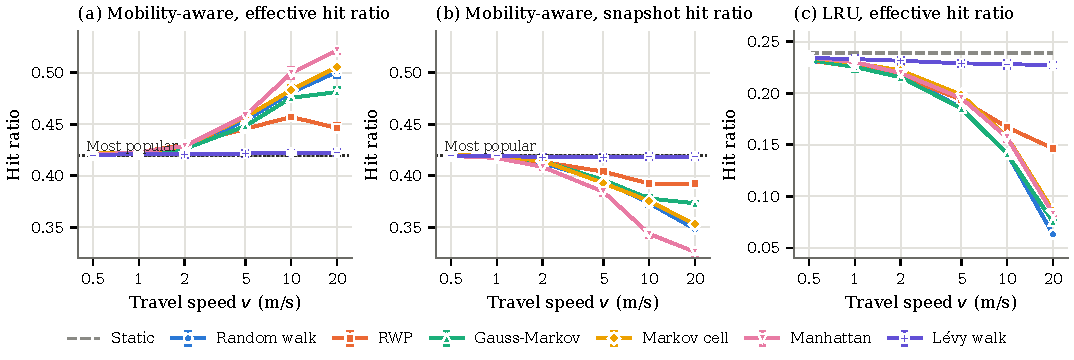
\includegraphics[width=\textwidth]{figures/fig_sbs_hit.pdf}
\caption{SBS caching. (a)--(c) Hit ratios against travel speed, mean of 10 seeds with 95\% confidence intervals; the dotted line is MPC (0.420). (d) Gain of the mobility-aware placement over MPC against the measured reach, one point per model and speed; the dotted reference line is fitted through the origin to all moving models except RWP.}
\label{fig:sbs}
\end{figure*}

\emph{Replication makes the gain immune to handovers.} Under MPC every SBS holds the same files, so any 10~s stay with any SBS completes the delivery. Its effective hit ratio is 0.418 to 0.420 under all models and speeds.

\emph{Diversity turns mobility into gain.} At 0.5~m/s the mobility-aware placement performs like MPC under every model (0.420 to 0.422). At 20~m/s its effective hit ratio is 0.522 under the Manhattan model, 0.505 under the Markov cell model, 0.501 under the random walk and 0.481 under Gauss-Markov, gains of 24.3\%, 20.4\%, 19.4\% and 15.1\% over MPC (Fig.~\ref{fig:sbs}a). Under RWP the gain peaks at 8.9\% at 10~m/s and falls to 6.4\% at 20~m/s; under the L\'evy walk it never exceeds 0.7\%.

\emph{Reach explains most of the spread.} Fig.~\ref{fig:sbs}d plots the gain of every model and speed against the reach. The correlation is 0.98, and for all moving models except RWP the gain grows by about 10.4\% for each additional SBS within reach. Nominal speed does not order the points; the L\'evy walk at 20~m/s has the reach (1.16) and the gain (0.7\%) of the other models at 1~m/s. RWP falls below the line. At 5~m/s it has the highest reach of all models (1.81) but a lower gain (6.2\%) than every model except the L\'evy walk. Its users concentrate in the center, so the cells they reach are mostly the same central cells: 56\% of the off-diagonal reach of $\mathbf{W}$ points to the central nine cells, against 38\% to 46\% for the other moving models (mean of 10 seeds). A central cache serves users from several neighbors and cannot complement each of them, so the reach of RWP buys less diversity. The gain therefore depends on how many caches a user reaches and on how evenly those caches are shared.

\emph{The snapshot metric reverses the conclusion.} The snapshot hit ratio of the same placement falls below MPC as speed grows, to 0.326 under the Manhattan model at 20~m/s, 22.3\% below MPC (Fig.~\ref{fig:sbs}b). A paper that reported only the snapshot ratio would conclude that the mobility-aware placement is worse than MPC, while the effective ratio shows it is 24.3\% better. The snapshot ratio counts only the cache at the request instant, so it penalizes a placement that relies on the next cells for the files it does not hold.

\emph{Reactive caching at the serving cell loses deliveries to handovers.} LRU serves a user only from the cell it is in at the request instant. Its effective hit ratio drops from 0.239 for static users to between 0.063 (random walk) and 0.146 (RWP) at 20~m/s, and stays at 0.227 under the L\'evy walk (Fig.~\ref{fig:sbs}c). Its snapshot ratio stays between 0.235 and 0.240 throughout, and the product of the snapshot ratio and the probability that a user stays at least $D_s$ in its current cell reproduces the effective ratio within 0.003 for every model and speed. The loss is thus the interruption mechanism of Section~\ref{subsec:mech-interrupt}, and it is set by one sojourn statistic.

\subsection{D2D Caching}
\label{subsec:res-d2d}

\begin{figure*}[t]
\centering
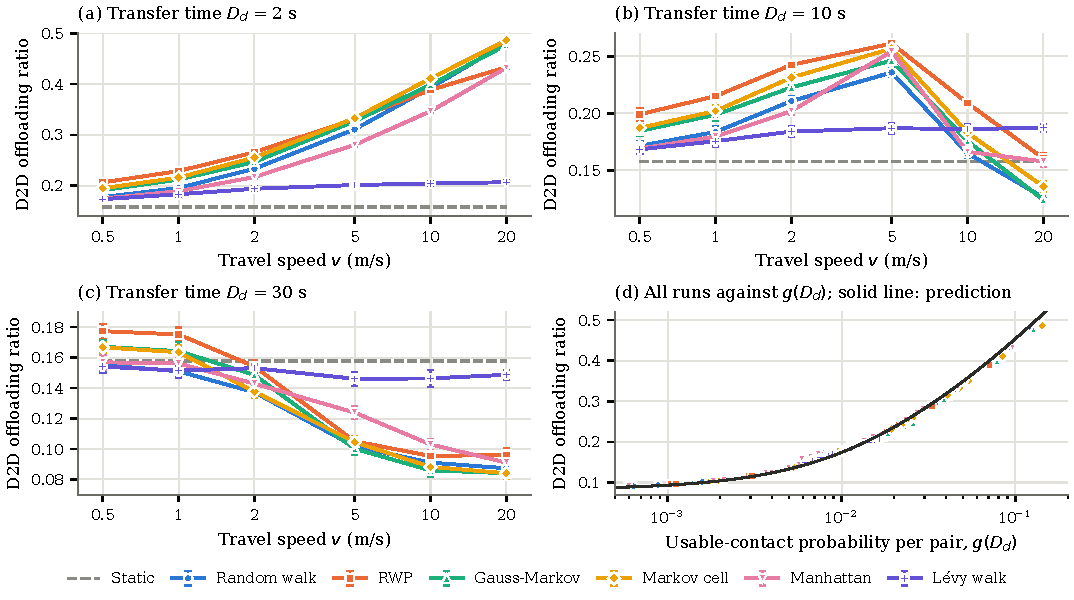
\includegraphics[width=\textwidth]{figures/fig_d2d.pdf}
\caption{D2D offloading. (a)--(c) Offloading ratio against travel speed for short, medium and long transfers, mean of 10 seeds with 95\% confidence intervals; the dashed line is the static network (0.158). (d) Offloading ratio of all 210 configurations (seven models, six speeds, five transfer times) against the usable-contact probability $g(D_d)$ of~\eqref{eq:gdd}; the solid line is the prediction~\eqref{eq:d2dpred}.}
\label{fig:d2d}
\end{figure*}

Fig.~\ref{fig:d2d}a--c reproduces the three conclusions found in the literature, in one setting, by changing only the transfer time.

\emph{Short transfers: mobility helps.} With $D_d=2$~s, offloading grows with speed under every moving model, from 0.158 for static users to between 0.432 (Manhattan) and 0.486 (Markov cell) at 20~m/s; the L\'evy walk reaches only 0.207. This agrees with the renewal-model result that offloading increases with speed~\cite{wang2018exploiting}.

\emph{Long transfers: mobility hurts.} With $D_d=30$~s, offloading falls with speed and, for every model except the L\'evy walk, drops to between 0.084 and 0.096 at 20~m/s, below the static network. At that speed contacts last 3 to 5~s on average. This agrees with the link-lifetime result that higher mobility lowers the success probability~\cite{jarray2016mobility}.

\emph{Medium transfers: the effect is non-monotone.} With $D_d=10$~s, offloading under every model except the L\'evy walk rises to between 0.236 and 0.261 at 5~m/s, where the mean contact lasts 12 to 20~s, and falls to between 0.124 and 0.161 at 20~m/s. Wang \emph{et al.} found a non-monotone dependence on speed in the optimal placement~\cite{wang2017mobility}; here it appears in the offloading ratio of a fixed placement.

\emph{One contact statistic predicts the offloading ratio.} These three regimes follow from a single quantity. Let $h_l$ be the number of contacts of length $l$ seconds per user pair over a period of $T$ seconds. If contacts form a stationary sequence, the probability that a pair offers at least $D_d$ consecutive seconds of contact within a window of $T_d$ seconds that starts at a random instant is approximately
\begin{equation}
g(D_d)=\frac{1}{T}\sum_{l\ge D_d} h_l\,\big[(l-D_d+1)+(T_d-D_d)\big].
\label{eq:gdd}
\end{equation}
The first term counts windows that open during a contact with at least $D_d$ seconds left; the second counts contacts long enough that start early enough in the window. Let $q_f$ be the probability that a user caches file $f$. If the $U-1$ other users act independently, the offloading ratio is
\begin{equation}
\rho=\sum_f p_f\Big[q_f+(1-q_f)\big(1-(1-g\,q_f)^{U-1}\big)\Big].
\label{eq:d2dpred}
\end{equation}
For static users $g$ is the fraction of pairs in range. We computed $g$ from the contact histogram of each run and compared~\eqref{eq:d2dpred} with the simulated ratio. Over the 210 configurations the mean absolute error is 0.004, 90\% of the errors are below 0.01, and the largest is 0.027, for the Markov cell model at 20~m/s with $D_d=2$~s, where many concurrent contacts make the independence assumption optimistic. All configurations fall on one curve (Fig.~\ref{fig:d2d}d): once $g(D_d)$ is known, neither the model nor the speed adds information.

Equation~\eqref{eq:gdd} also explains the crossover. For a short transfer, $g$ is close to the contact rate times $T_d$ and grows with speed. For a long one, only contacts longer than $D_d$ count, and their number falls as speed shortens contacts. The L\'evy walk is flat because its long pauses keep contacts long at every speed, and RWP gives the highest offloading among the moving models at low speed because its central concentration raises the contact rate. A mobility model therefore enters D2D caching only through its contact-length distribution, which can be measured from a trace and reported in a paper.

\subsection{Training on the Wrong Model}
\label{subsec:mismatch}

\begin{table}[t]
\centering
\caption{Effective hit ratio when the mobility-aware placement is trained on one model (rows) and used under another (columns), $v=5$~m/s, mean of 10 seeds. MPC gives 0.420 in every column.}
\label{tab:mismatch}
\footnotesize
\renewcommand{\arraystretch}{1.1}
\setlength{\tabcolsep}{2.6pt}
\begin{tabular}{lccccccc}
\hline
Train $\backslash$ Test & Stat. & RW & RWP & GM & MC & MH & L\'evy \\
\hline
Static & \textbf{.420} & .420 & .420 & .420 & .420 & .420 & .420 \\
Random walk & .394 & \textbf{.454} & .451 & .449 & .453 & .457 & .404 \\
RWP & .398 & .446 & \textbf{.445} & .444 & .449 & .451 & .409 \\
Gauss-Markov & .399 & .450 & .450 & \textbf{.448} & .454 & .454 & .409 \\
Markov cell & .391 & .451 & .449 & .449 & \textbf{.457} & .457 & .404 \\
Manhattan & .385 & .451 & .449 & .449 & .452 & \textbf{.458} & .397 \\
L\'evy walk & .418 & .434 & .434 & .434 & .436 & .436 & \textbf{.421} \\
\hline
\end{tabular}
\end{table}

Table~\ref{tab:mismatch} trains the mobility-aware placement on one model and uses it under another, at 5~m/s. Training on static users reproduces MPC, as it should, since $\mathbf{W}$ is then the identity. The 95\% confidence half-width of every entry is below 0.006.

Among the five models in which users keep moving, mismatch costs little: in every column, the worst cross-model entry is within 0.009 of the matched one. In the RWP column every cross-trained placement does better than the one trained on RWP (0.449 to 0.451 against 0.445). This is the effect seen in Fig.~\ref{fig:sbs}d from the other side: RWP reach is concentrated on shared central cells, which~\eqref{eq:maobj} treats as independent visits, so a placement learned from more uniform movement spreads content better.

Mismatch is costly when the training model moves and the actual users mostly do not. A placement trained on any of the five moving models and used with static users gives 0.385 to 0.399, 5.0\% to 8.2\% below MPC; used with L\'evy walkers it gives 0.397 to 0.409, again below MPC. Training on the L\'evy walk is safe but timid: it is never more than 0.002 below MPC, and on moving users it gives 0.434 to 0.436 against 0.445 to 0.458 for the matched placements. What matters is therefore the regime, moving or pause-dominated, more than the model. A mobility-aware placement should be trained on mobility of the same regime as its users, and when the population mixes both, it should be checked against the oblivious baseline, because a diversity-seeking placement can do worse than MPC for users who stay put.
